\documentclass[a4paper,11pt]{article}
\usepackage[margin=1.1in]{geometry}
\usepackage{f420}
\usepackage{modules/braid}

\title{ }
\author{ }
\date{\today}

\begin{document} \maketitle

\section{Definitions}

\begin{definition}
	\emph{A Voronoi diagram} is a subdivision of a \(n \times m\) table equipped with a greedy braid into regions such that
   \begin{enumerate}
	\item Left boundary of each region is composed of a single braid strand and possibly a piece of the boundary;
	\item Right boundary of each region is composed of several pieces \(e_1, e_2, \ldots, e_k\) of braid strands, such that \begin{enumerate}
	   \item the pieces \(e_1, e_2, \ldots, e_k\) cross no strand from left to right,
	   \item the strand containing \(e_i\) crosses the strand containing \(e_{i+1}\) from left to right at the point where \(e_i\) meets \(e_{i+1}\), \(i = 1,\ldots, k-1\).
	\end{enumerate}
   \end{enumerate}
\end{definition}

\begin{lemma}
	The following are equivalent:
   \begin{enumerate}
	\item Point \(p\) belongs to the Voronoi cell \(f_i\) of a Voronoi site \(s_i\);
	\item Site \(s_i\) is the leftmost site such that there is a path from \(s_i\) to \(p\) that crosses no braid strand from left to right.
   \end{enumerate}
\end{lemma}

\section{Notation}

\newcommand{\VD}{\ensuremath{\text{\sffamily VD}}\xspace}
\newcommand{\braid}{\ensuremath{\mathcal{B}}\xspace}

\begin{enumerate}
	\item \(\braid\) for the greedy braid of the \(\frac{n}{2} \times m\) table;
	\item \(\VD\) for the Voronoi diagram of \(\braid\) % the \(\frac{n}{2} \times m\) table;
	\item \(\braid^*\) for the upward \(\frac{n}{2} \times m\) greedy braid;
	\item \(\braid^{-h}\) for the \(\lr*{\frac{n}{2} + h} \times m\) greedy braid that starts \(h\) rows above the middle line;
	\item \(\VD^{-h}\) for the Voronoi diagram corresponding to \(\braid^{-h}\);
	\item \(s_0, \ldots, s_{m+n}\) for the sites of the Voronoi diagram;
	\item \(f_0, \ldots, f_{m+n}\); \(f_0^{-h}, \ldots, f_{m+n}^{-h}\) for the Voronoi cells of \(\VD\) and \(\VD^{-h}\) correspondingly;
	\item \(c_0, \ldots, c_{m+n}\); \(c_0^{-h}, \ldots, c_{m+n}^{-h}\) for the lower right corners of the Voronoi cells of \(\VD\) and \(\VD^{-h}\) correspondingly.
\end{enumerate}


\begin{figure}[ht] \centering
	\begin{tikzpicture}[scale=0.65]
	\draw
	\foreach \h / \t in {0 / A, 1 / A, 2 / C, 3 / C}
		{(-0.6,3.5-\h) node{{\sffamily\t}}}
	\foreach \w / \t in {0 / A, 1 / A, 2 / C, 3 / B, 4 / A, 5 / C}
		{(0.4+\w,4.5) node{{\sffamily\t}}};
 % ────── Границы областей Вороного
	\fill[c8,opacity=0.22] (0,0)\vr\vu\vl -- cycle;
	\fill[c9,opacity=0.22] (0,1)\vd\vr\vuu\vl -- cycle;
	\fill[ca,opacity=0.22] (0,2)\vd\vr\vu\vul -- cycle;
	\fill[cb,opacity=0.22] (0,3)\vd\vrd\vdd\vdd\vrr
		\vuu\vuu\vul\vlu\vul -- cycle;
	\fill[c1,opacity=0.22] (0,4)\vd\vrd\vdr\vrd\vdd\vdd\vrr\vrr
		\vu\vuu\vl\vlu\vu\vl\vlu\vul\vlu -- cycle;
	\fill[c2,opacity=0.22] (0.5,4)\vdr\vrd\vdr\vr\vuu\vl\vlu -- cycle;
	\fill[c3,opacity=0.22] (1.5,4)\vdr\vr\vu -- cycle;
	\fill[c4,opacity=0.22] (2.5,4)\vdd\vdd\vdr\vr\vuu\vuu\vu -- cycle;
	\fill[c5,opacity=0.22] (3.5,4)\vdd\vdd\vdd\vdd\vrr\vrr\vr
		\vuu\vu\vlu\vuu\vu\vl\vlu -- cycle;
	\fill[c6,opacity=0.22] (4.5,4)\vdr\vr\vu -- cycle;
	\fill[c7,opacity=0.22] (5.5,4)\vdd\vdd\vdr\vuu\vuu\vu -- cycle;
 % ────── Нити кос
	\draw[thick,green] (0,3.5)
	\hc\hc\hx\hx\hc\hx\hn
	\hc\hc\hx\hx\hc\hx\hn
	\hx\hx\hc\hx\hc\hc\hn
	\hx\hx\hc\hx\hx\hc;
 % ────── Диагональные рёбра
	\draw[thick,red]
	\foreach \x / \y in
		{0 / 3, 0 / 4, 1 / 3, 1 / 4,
		 2 / 1, 2 / 2, 4 / 3, 4 / 4,
		 5 / 1, 5 / 2}
		{(\x,\y) -- ++(1,-1)};
 % ────── Границы рисунка
	\draw[black,opacity=0.35] (0,0) grid (6,4);
	\draw (0,0) rectangle (6,4);
 % ────── Сайты и углы областей
	\draw
	\foreach \i / \ix / \iy in
		{1/3.5/0, 2/2.5/2.5, 3/2.5/3.5, 4/3.5/1.5,
		 5/6/0, 6/5.5/3.5, 7/6/1.5}
		{(-1+\i,4) node[circle,fill=c\i,inner sep=0.55mm]{ }
		 (\ix,\iy) \rdcor{\i}}
	\foreach \nom / \i / \ix / \iy in
		{0/8/0.5/0, 1/9/0.5/0.5, 2/a/0.5/1.5, 3/b/1.5/0}
		{(0,\nom) node[circle,fill=c\i,inner sep=0.55mm]{ }
		 (\ix,\iy) \rdcor{\i}};

 % ══════════════════

   \begin{scope}[xshift=8.5cm]
	\draw
	\foreach \h / \t in {0 / A, 1 / A, 2 / C, 3 / B,
	                     4 / A, 5 / A, 6 / C, 7 / C}
		{(-0.6,7.5-\h) node{{\sffamily\t}}}
	\foreach \w / \t in {0 / A, 1 / A, 2 / C, 3 / B, 4 / A, 5 / C}
		{(0.4+\w,8.5) node{{\sffamily\t}}};
 % ────── Границы областей Вороного
	\fill[c8,opacity=0.22] (0,0)\vr\vu\vl -- cycle;
	\fill[c9,opacity=0.22] (0,1)\vd\vr\vuu\vl -- cycle;
	\fill[ca,opacity=0.22] (0,2)\vd\vr\vu\vul -- cycle;
	\fill[cb,opacity=0.22] (0,3)\vd\vrd\vdd\vdd\vrr
		\vuu\vuu\vul\vlu\vul -- cycle;
	\fill[c1,opacity=0.22] (0,4)\vd\vrd\vdr\vrd\vdd\vdd\vrr\vrr
		\vuu\vul\vlu\vu\vl\vlu\vul\vlu -- cycle;
	\fill[c2,opacity=0.22] (0.5,4)\vdr\vrd\vdr\vr\vu\vul\vlu -- cycle;
	\fill[c3,opacity=0.22] (1.5,4)\vdr\vrd\vdd\vdr\vrd\vdd\vrr\vrr\vr
		\vu\vlu\vul\vlu\vul\vlu\vul\vlu -- cycle;
	\fill[c4,opacity=0.22] (2.5,4)\vdr\vrd\vdr\vrd\vdr\vrd\vdr
		\vuu\vlu\vu\vl\vlu\vul\vlu -- cycle;
	\fill[c5,opacity=0.22] (3.5,4)\vdr\vrd\vdr\vr\vu\vul\vlu -- cycle;
	\fill[c6,opacity=0.22] (4.5,4)\vdr\vrd\vdd\vdr\vuu\vuu\vlu -- cycle;
	\fill[c7,opacity=0.22] (5.5,4)\vdr\vu -- cycle;
 % ────── Нити кос
	\draw[thick,green] (0,5.5)
	\hx\hx\hc\hx\hx\hc\hn
	\hx\hx\hx\hc\hx\hc\hn
	\hc\hc\hc\hc\hc\hc\hn
	\hc\hc\hx\hc\hc\hx\hn
	\hx\hx\hc\hc\hc\hc\hn
	\hx\hx\hc\hx\hx\hc;
 % ────── Диагональные рёбра
	\draw[thick,red]
	\foreach \x / \y in
		{0 / 3, 0 / 4, 1 / 3, 1 / 4,
		 2 / 1, 2 / 2, 4 / 3, 4 / 4,
		 5 / 1, 5 / 2,
		 2 / 6, 3 / 5, 5 / 6}
		{(\x,\y) -- ++(1,-1)};
 % ────── Границы рисунка
	\draw[black,opacity=0.35] (0,0) grid (6,8);
	\draw (0,0) rectangle (6,8);
	\draw (0,6) -- (6,6);
 % ────── Сайты и углы областей
	\draw
	\foreach \i / \ix / \iy in
		{1/3.5/0, 2/2.5/2.5, 3/6/0, 4/6/0.5,
		 5/5.5/2.5, 6/6/1.5, 7/6/3.5}
		{(-1+\i,4) node[circle,fill=c\i,inner sep=0.55mm]{ }
		 (\ix,\iy) \rdcor{\i}}
	\foreach \nom / \i / \ix / \iy in
		{0/8/0.5/0, 1/9/0.5/0.5, 2/a/0.5/1.5, 3/b/1.5/0}
		{(0,\nom) node[circle,fill=c\i,inner sep=0.55mm]{ }
		 (\ix,\iy) \rdcor{\i}};
   \end{scope}

   \begin{scope}[xshift=3cm,yshift=6.5cm,rotate=45]
	\draw[<->,gray] (-1.8,0) -- (1.8,0);
	\draw (0.65,0.2) node[rotate=45,text depth=0.8ex]{{\footnotesize Right}}
	     (-0.75,0.2) node[rotate=45,text depth=0.8ex]{{\footnotesize Left}};
   \end{scope}

	\draw (3,-1) node{(a)} (11.5,-1) node{(b)};
\end{tikzpicture}


	\begin{tikzpicture}[scale=0.65]
	\draw
	\foreach \h / \t in {0 / A, 1 / A, 2 / C, 3 / C}
		{(-0.6,3.5-\h) node{{\sffamily\t}}}
	\foreach \w / \t in {0 / A, 1 / A, 2 / C, 3 / B, 4 / A, 5 / C}
		{(0.4+\w,4.5) node{{\sffamily\t}}};
 % ────── Границы областей Вороного
	\fill[c8,opacity=0.22] (0,0)\vr\vu\vl -- cycle;
	\fill[c9,opacity=0.22] (0,1)\vd\vr\vuu\vl -- cycle;
	\fill[ca,opacity=0.22] (0,2)\vd\vr\vu\vul -- cycle;
	\fill[cb,opacity=0.22] (0,3)\vd\vrd\vdd\vdd\vrr
		\vuu\vuu\vul\vlu\vul -- cycle;
	\fill[c1,opacity=0.22] (0,4)\vd\vrd\vdr\vrd\vdd\vdd\vrr\vrr
		\vu\vuu\vl\vlu\vu\vl\vlu\vul\vlu -- cycle;
	\fill[c2,opacity=0.22] (0.5,4)\vdr\vrd\vdr\vr\vuu\vl\vlu -- cycle;
	\fill[c3,opacity=0.22] (1.5,4)\vdr\vr\vu -- cycle;
	\fill[c4,opacity=0.22] (2.5,4)\vdd\vdd\vdr\vr\vuu\vuu\vu -- cycle;
	\fill[c5,opacity=0.22] (3.5,4)\vdd\vdd\vdd\vdd\vrr\vrr\vr
		\vuu\vu\vlu\vuu\vu\vl\vlu -- cycle;
	\fill[c6,opacity=0.22] (4.5,4)\vdr\vr\vu -- cycle;
	\fill[c7,opacity=0.22] (5.5,4)\vdd\vdd\vdr\vuu\vuu\vu -- cycle;
 % ────── Нити кос
	\draw[thick,green] (0,3.5)
	\hc\hc\hx\hx\hc\hx\hn
	\hc\hc\hx\hx\hc\hx\hn
	\hx\hx\hc\hx\hc\hc\hn
	\hx\hx\hc\hx\hx\hc;
 % ────── Диагональные рёбра
	\draw[thick,red]
	\foreach \x / \y in
		{0 / 3, 0 / 4, 1 / 3, 1 / 4,
		 2 / 1, 2 / 2, 4 / 3, 4 / 4,
		 5 / 1, 5 / 2}
		{(\x,\y) -- ++(1,-1)};
 % ────── Границы рисунка
	\draw[black,opacity=0.35] (0,0) grid (6,4);
	\draw (0,0) rectangle (6,4);
 % ────── Путь, не пересекающий нити дважды
	\draw[thick,DarkOrchid] (2,4) -- (2,2) -- (3,1) -- (5,1) -- (6,0);
	\draw[thick,DarkOrchid] (3,4) -- (6,1) -- (6,0.5);
	\fill[black] (4,1) circle[radius=1mm] node[anchor = north east]{\small \(p_1\)};
	\fill[black] (4,3) circle[radius=1mm] node[anchor = north east]{\small \(p_2\)};
 % ────── Сайты и углы областей
	\draw
	\foreach \i / \ix / \iy in
		{1/3.5/0, 2/2.5/2.5, 3/6/0, 4/6/0.5,
		 5/5.5/2.5, 6/6/1.5, 7/6/3.5}
		{(-1+\i,4) node[circle,fill=c\i,inner sep=0.55mm]{ }
		 (\ix,\iy) \rdcor{\i}}
	\foreach \nom / \i / \ix / \iy in
		{0/8/0.5/0, 1/9/0.5/0.5, 2/a/0.5/1.5, 3/b/1.5/0}
		{(0,\nom) node[circle,fill=c\i,inner sep=0.55mm]{ }
		 (\ix,\iy) \rdcor{\i}};

 % ══════════════════

	\draw (3,-1) node{(c)};
\end{tikzpicture}


	\caption{(a) Voronoi diagram for a given greedy braid, (b) \(\VD^{-2}\), (c) paths from \(s_6\) to \(c_6^{-2}\) through \(p_1\) and from \(s_7\) to \(c_7^{-2}\) through \(p_2\)}
	\label{fig:vd-ex}
\end{figure}


\section{Query}

\begin{problem}
	Given braid \braid, the lower right corners \(c_0^{-h}, \ldots, c_{m+n}^{-h}\) of the Voronoi cells of \(\VD^{-h}\), point \(p\) and a number \(i\), check whether \(p \in f_i^{-h}\), \(p\) is to the left or to the right from \(f_i^{-h}\).
\end{problem}

\begin{lemma}
	The following are equivalent:
   \begin{enumerate}
	\item Point \(p\) belongs to the Voronoi cell \(f_i^{-h}\) of \(\VD^{-h}\);
	\item There is a path from \(s_i\) to \(c_i^{-h}\) passing through \(p\) that crosses no strand of \braid twice.
   \end{enumerate}
\end{lemma}

The path can utilize diagonal edges, see Figure~\ref{fig:vd-ex},~(c): \(p_1 \in f_6^{-2}\) (green), \(p_2 \in f_7^{-2}\) (yellow).

\newpage

\subsection{Entanglement of triples oracle}

\begin{definition}
	We call two triples of numbers \(\lr*{a_1, a_2, a_3}\),
	\(\lr*{b_1, b_2, b_3}\) \emph{entangled} if
	\[ a_1 < b_1,\ a_2 > b_2,\ a_3 < b_3\quad\text{or}\quad
	   a_1 > b_1,\ a_2 < b_2,\ a_3 > b_3\]
\end{definition}

\begin{theorem} \label{thm:entgtripls}
	There exists a data structure that can store a set of \(n\) triples
	\[S = \set*{\lr*{a^1_1, a^1_2, a^1_3}, \ldots, \lr*{a^n_1, a^n_2, a^n_3}}\]
	and, given a query triple \(q = \lr*{q_1, q_2, q_3}\), output
	in time \(\Ot\lr*{1}\)  %  Count logs precisely
	the number of triples in \(S\) that are entangled with \(q\).
\end{theorem}

\begin{proof}
	Store the set \(S\) in a 3-dimensional range tree [{\color{magenta} cite!}].
	A \(d\)-dimensional range tree is a data structure that stores several points
	in \(\mathbb{R}^d\) and effectively reports all the stored points that are
	inside a \(d\)-dimensional rectangular parallelepiped defined by
	its lower and higher coordinates on each axis.

\begin{figure}[ht] \centering
	\begin{tabular}{ccc}
\makecell[c]{\begin{tikzpicture}[xscale=0.6,yscale=-0.6]
	\fill[cb,opacity=0.25] (0,0) rectangle (6,4);
	\draw (0,0) rectangle (6,4)
	      (0,2.25) -- (6,2.25) (0,3.5) -- (6,3.5)
	      (2,0) -- (4.25,3.5);
	\draw[thick,green] (3.75,0)
	      .. controls (3.75,1) and (2.25,1.5) ..
	      (2.25,2.25)
	      .. controls (2.25,3) and (5.25,2.75) ..
	      (5.25,3.5);
	\fill[black]
	 (2,0) circle[fill=black,radius=1mm]
	       node[anchor = south west]{\small \(s_i\)}
	 (3.4464,2.25) circle[radius=1mm]
	               node[anchor = south west]{\small \(p\)}
	 (4.25,3.5) circle[radius=1mm]
	            node[anchor = south west]{\small \(c_i^{-h}\)};
\end{tikzpicture}} & \hspace{0.8cm} &
\makecell[c]{\begin{tikzpicture}[xscale=0.45,yscale=0.5]
 % ────── Задняя часть
	\draw[dashed,thick,->,IndianRed] \proj000 -- \proj070;
	\draw[dashed] \proj050 -- \proj000 \proj050 -- \proj054
	              \proj050 -- \proj650
	              \proj23{2.5} -- \proj234 \proj23{2.5} -- \proj63{2.5}
	              \proj23{2.5} -- \proj20{2.5};
 % ────── Отсечения сзади
	\draw[thick,HotPink,dotted]
	      \proj254 -- \proj250 -- \proj200
	      \proj65{2.5} -- \proj05{2.5} -- \proj00{2.5}
	      \proj630 -- \proj030 -- \proj034;
 % ────── Поверхность парал-пипеда
	\filldraw[draw=black,fill=cb,fill opacity=0.3]
	   \proj000 -- \proj600 -- \proj650 --
	   \proj654 -- \proj054 -- \proj004 -- cycle;
	\fill[c3,opacity=0.7] \proj20{2.5} -- \proj60{2.5} --
	                      \proj63{2.5} -- \proj63{2.5} --
	                      \proj634 -- \proj234 -- \proj204 -- cycle;
	\draw \proj604 -- \proj004 \proj604 -- \proj654 \proj604 -- \proj600;
 % ────── Координатные оси
	\draw[thick,->,IndianRed] \proj000 -- \proj800;
	\draw[thick,->,IndianRed] \proj000 -- \proj00{5.5};
 % ────── Отсечения на поверхности
	\draw[thick,HotPink] \proj254 -- \proj204 -- \proj200
	      node[anchor=north east]{\color{black}\small \(s_i\)}
	      \proj65{2.5} -- \proj60{2.5} -- \proj00{2.5}
	      node[anchor=east]{\color{black}\small \(c_i^{-h}\)}
	      \proj630 -- \proj634 -- \proj034
	      node[anchor=south east]{\color{black}\small \(p\)};
\end{tikzpicture}} \\
	(a) & & (b) \\
\end{tabular}


	\caption{(a) A triple \(\lr*{a^i_1, a^i_2, a^i_3}\) entangled
	with \(\lr*{q_1, q_2, q_3}\),
	         (b) a range query that finds this triple}
	\label{fig:paral-trans}
\end{figure}

	An entanglement query can then be interpreted as two 3-dimensional range
	queries, as shown in Figure~\ref{fig:paral-trans}:
   \begin{enumerate}
	\item \(a_1 < q_1,\ a_2 > q_2,\ a_3 < q_3\) is a 3-dimensional parallelepiped
	  to the left, further and lower than the point \(\lr*{q_1, q_2, q_3}\)
	  (call this \emph{left entanglement query});
	\item \(a_1 > q_1,\ a_2 < q_2,\ a_3 > q_3\) is a 3-dimensional parallelepiped
	  to the right, closer and higher than the point \(\lr*{q_1, q_2, q_3}\)
	  (call this \emph{right entanglement query}).
   \end{enumerate}
\end{proof}

\begin{remark}
	The construction of a 3-dimensional range tree takes \(O \lr*{n \log^2 n}\) time,
	and a range query takes \(O \lr*{\log n}\) time.
\end{remark}


\subsection{Entanglement of strands oracle}

\begin{theorem} \label{thm:entgstrands}
	There exists a data structure that can store a reduced embedded braid \braid and,
	given an arbitrary point triple \(g = (0,r)\), \(h = (k,s)\), \(f = (\ell,t)\),
	decide in time \(\Ot\lr*{1}\) if there exists a path from \(g\) to \(f\)
	through \(h\) that is not double-crossed by any strand.
\end{theorem}

\begin{proof}
	To build the data structure, first partition the grid of height \(n\)
	hierarchically into \(O\lr*{n}\) canonical strips located in a binary tree:
	each canonical strip contains two canonical strips of half its height.

	For each canonical strip \(\lr*{a, b}\) build an entanglement of triples
	oracle (Theorem~\ref{thm:entgtripls}): for each strand \(s\) store the triple
	\(\lr*{s_0, s_a, s_b}\) of its positions at the ground of the grid,
	the top of the canonical strip, and the bottom of
	the canonical strip respectively.

	In total there are \(O\lr*{n}\) entanglement of triples oracles,
	the construction of them takes \(O\lr*{n^2 \log^2 n}\) time.

\begin{figure}[ht] \centering
      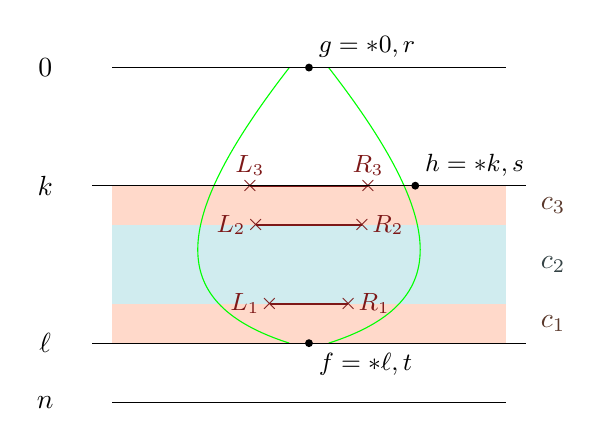
\begin{tikzpicture}[yscale=-0.5,xscale=0.5]
	\fill[LightSalmon,opacity=0.4] (-5,3) rectangle (5,4);
	\fill[PowderBlue, opacity=0.6] (-5,4) rectangle (5,6);
	\fill[LightSalmon,opacity=0.4] (-5,6) rectangle (5,7);
	\draw[LightSalmon!35!black] (6.2,6.5) node{\(c_1\)};
	\draw[PowderBlue!30!black]  (6.2,  5) node{\(c_2\)};
	\draw[LightSalmon!35!black] (6.2,3.5) node{\(c_3\)};

	\draw[green] ( 0.5,0) .. controls ( 3.6,4) and ( 3.6,6) .. ( 0.5,7)
	             (-0.5,0) .. controls (-3.6,4) and (-3.6,6) .. (-0.5,7);
	
	\draw[FireBrick!70!black,thick]
	  (-1,6)      node{\footnotesize \(\times\)} node[left]{\small \(L_1\)}
	  -- (1,6)    node{\footnotesize \(\times\)} node[right]{\small \(R_1\)}
	  (-1.35,4)   node{\footnotesize \(\times\)} node[left]{\small \(L_2\)}
	  -- (1.35,4) node{\footnotesize \(\times\)} node[right]{\small \(R_2\)}
	  (-1.5,3)    node{\footnotesize \(\times\)} node[above]{\small \(L_3\)}
	  -- (1.5,3)  node{\footnotesize \(\times\)} node[above]{\small \(R_3\)};

	\draw (-5,0) -- (5,0) (-5.5,3) -- (5.5,3) (-5.5,7) -- (5.5,7) (-5,8.5) -- (5,8.5);
	\fill[black]
	 (0,0) circle[radius=1mm]
	             node[anchor = south west]{\small \(g = \lr*{0, r}\)}
	 (2.7,3) circle[radius=1mm]
	             node[anchor = south west]{\small \(h = \lr*{k, s}\)}
	 (0,7) circle[radius=1mm]
	             node[anchor = north west]{\small \(f = \lr*{\ell, t}\)};
	\draw (-6.7,0) node{\(0\)}  (-6.7,3) node{\(k\)}
	      (-6.7,7) node{\(\ell\)}  (-6.7,8.5) node{\(n\)};
   \end{tikzpicture}

   \caption{The decomposition of the strip~\(\lr*{k, \ell}\) into canonical strips;
            boundaries \(\lr*{L_i, R_i}\) of entanglement-free regions} 
   \label{fig:eostrands}
\end{figure}

	To answer the query, decompose the strip~\((k,\ell)\) into
	canonical strips~\(c_1, c_2, \ldots, c_v\), the indexation is from the bottom
	of the strip upwards (see Figure~\ref{fig:eostrands}). At each
	boundary of neighboring canonical strips~\(c_i\), \(c_{i+1}\) we maintain
	an \emph{entanglement-free region}~\(\left[ L_i, R_i \right]\) which is
	the region where the not-double-crossed path can pass through.

	It is obvious that at least one such path from~\(g\) to \(f\) exists, therefore
	each entanglement-free region is nonempty. Naturally, \(L_0 = R_0 = f\).
	Points~\(L_{i+1}, R_{i+1}\) are constructed from \(L_i, R_i\) recursively:
   \begin{enumerate}
	\item \(L_{i+1}\) is the leftmost point such that any strand that is
	  to the left of \(g\) and \(L_i\) is also to the left of \(L_{i+1}\),
	\item \(R_{i+1}\) is the rightmost point such that any strand that is
	  to the right of \(g\) and \(R_i\) is also to the right of \(R_{i+1}\).
   \end{enumerate}
	Given \(L_i\), we find \(L_{i+1}\) using binary search in the boundary
	of~\(c_{i+1}, c_{i+2}\): if for a point~\(p\) the left entanglement query
	for~\(\lr*{g, p, L_i}\) returns some strands, descend to the right,
	otherwise descend to the left.
	Given \(R_i\), we find \(R_{i+1}\) in a symmetric way.

\begin{lemma} \label{lm:entg}
	The recursive construction of~\(L_i, R_i\) is correct;
	the following are equivalent:
   \begin{itemize}
	\item[a)] a point \(p\) is to the left of \(L_i\),
	\item[b)] there exists a strand that is to the left of \(g\) and \(f\),
	  but to the right of \(p\).
   \end{itemize}
\end{lemma}

\begin{proof} \begin{itemize}
	\item \( \text{b)} \Rightarrow \text{a)} \): Assume that \(p\) is
	to the right of (or equal to) \(L_i\), see Figure~\ref{fig:entga}.
	The strand~\(\sigma\), which is to the left of~\(g\) and~\(f\), but
	to the right of~\(p\), is also to the right of~\(L_i\); this contradicts
	the construction of~\(L_i\). 

\begin{figure}[ht] \centering
      \begin{subfigure}[t]{0.36\textwidth} \centering
      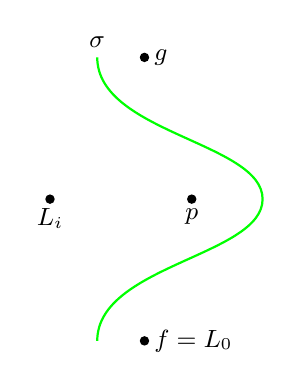
\begin{tikzpicture}[scale=0.6]
	\fill[black]
	(2,0) circle[radius=1mm]
	  node[right]{\small \(f = L_0\)}
	(0,3) circle[radius=1mm]
	  node[below]{\small \(L_i\)}
	(3,3) circle[radius=1mm]
	  node[below]{\small \(p\)}
	(2,6) circle[radius=1mm]
	  node[right]{\small \(g\)};
	\draw[thick,green] (1,6) .. controls (1,4.4) and (4.5,4.2) ..
	                   (4.5,3) .. controls (4.5,1.8) and (1,1.6) .. (1,0);
	\draw (1,6) node[above]{\small \(\sigma\)};
      \end{tikzpicture}
      \caption{ }
      \label{fig:entga}
   \end{subfigure}\hspace{0.4cm}
   \begin{subfigure}[t]{0.36\textwidth} \centering
      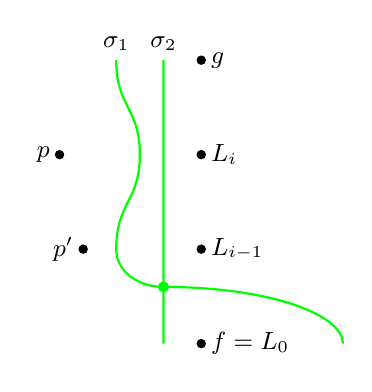
\begin{tikzpicture}[scale=0.6]
	\fill[black]
	(3,0) circle[radius=1mm]
	  node[right]{\small \(f = L_0\)}
	(3,2) circle[radius=1mm]
	  node[right]{\small \(L_{i-1}\)}
	(3,4) circle[radius=1mm]
	  node[right]{\small \(L_i\)}
	(3,6) circle[radius=1mm]
	  node[right]{\small \(g\)}
	(0.5,2) circle[radius=1mm]
	  node[left]{\small \(p^\prime\)}
	(0,4) circle[radius=1mm]
	  node[left]{\small \(p\)};
	\draw[thick,green] (2.2,0) -- (2.2,6)
	  (1.2,6) .. controls (1.2,5) and (1.7,5) ..
	  (1.7,4) .. controls (1.7,3) and (1.2,3) ..
	  (1.2,2) .. controls (1.2,1.5) and (1.7,1.2) ..
	  (2.2,1.2) node[circle,fill=green,inner sep=0.5mm]{ }
	  .. controls (4.5,1.2) and (6,0.6) .. (6,0);
	\draw (1.2,6) node[above]{\small \(\sigma_1\)}
	      (2.2,6) node[above]{\small \(\sigma_2\)};
      \end{tikzpicture}
      \caption{ }
      \label{fig:entgb}
   \end{subfigure}\hspace{0.4cm}

   \caption{Proof of Lemma~\ref{lm:entg}}
\end{figure}

	\item \( \text{a)} \Rightarrow \text{b)} \): Proof by induction in~\(i\);
	assume there are no strands that are to the left of~\(g\) and~\(f\),
	but to the right of~\(p\). There is however a strand~\(\sigma_1\)
	between~\(L_i\) and~\(p\) that made us descend to the right when performing
	the binary search for~\(L_i\); \(\sigma_1\) is to the left of~\(L_{i-1}\),
	see Figure~\ref{fig:entgb}. The strand~\(\sigma_1\) must be
	to the right of~\(f\), since it is to the left of~\(g\)
	and to the right of~\(p\).

	Take a point~\(p^\prime\) immediately to the left of~\(\sigma_1\)
	at the level of~\(L_{i-1}\). By the induction hypothesis, there exists a strand
	that is to the left of~\(g\) and~\(f\), but to the right of~\(p^\prime\),
	call it \(\sigma_2\). The strand~\(\sigma_2\) must cross \(\sigma_1\)
	below~\(p^\prime\), since \(\sigma_2\) is to the left of~\(f\), and \(p^\prime\)
	is the immediate left neighbor of~\(\sigma_1\).

	Since the braid is reduced, \(\sigma_2\) is to the right of~\(p\);
	this contradicts the assumption for~\(p\).
\end{itemize} \end{proof}

	Lemma~\ref{lm:entg} implies that there exists a path from~\(g\) to~\(f\)
	through~\(h\) that is not double-crossed by any strand if and only if \(h\)
	is between~\(L_v\) and~\(R_v\). Moreover, if \(h\) is outside the
	entanglement-free region, we can conclude whether there is a right or left
	entanglement of the \(g\)-to-\(h\)-to-\(f\) path with a strand of~\braid.
	
\begin{remark}
	The strip~\(\lr*{k, \ell}\) is decomposed into~\(O\lr*{\log n}\)
	canonical strips, therefore there is as much entanglement-free regions
	to be calculated. For each region~\(\lr*{L_i, R_i}\) two binary searches
	with~\(O\lr*{\log n}\) probes are done. Each probe calls a range query
	that takes \(O\lr*{\log n}\) time. In total, the entanglement of strands
	query takes \(O\lr*{\log^3 n}\) time.
\end{remark}
\end{proof}

%\bibliography{}{}
%\bibliographystyle{plain}

\end{document}
